\documentclass[tikz,border=4pt]{standalone}
\usepackage{tikz}
\usetikzlibrary{shapes.geometric}

\begin{document}
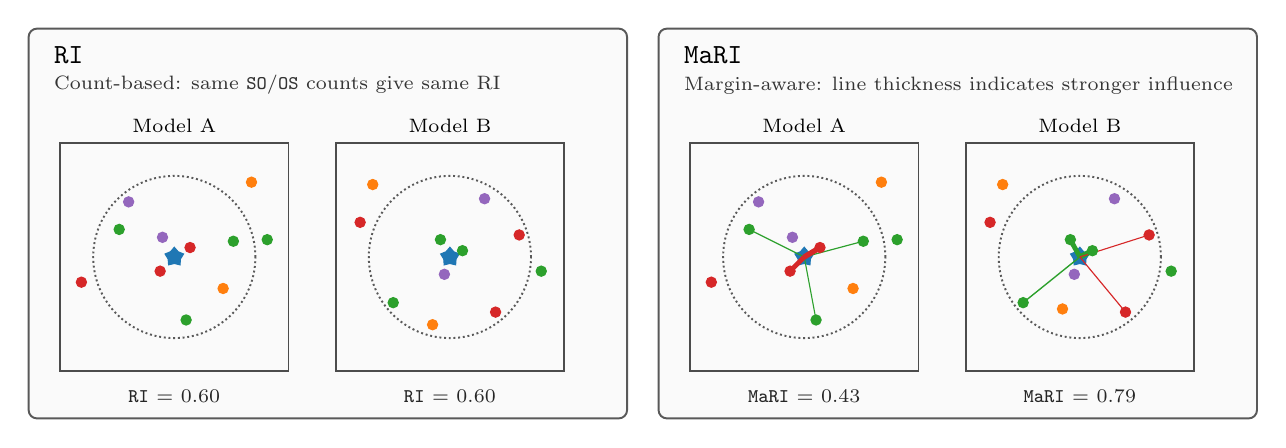
\begin{tikzpicture}[font=\small]
  \definecolor{anchorblue}{RGB}{31,119,180}
  \definecolor{sscol}{RGB}{148,103,189}
  \definecolor{oocol}{RGB}{255,127,14}
  \definecolor{socol}{RGB}{44,160,44}
  \definecolor{oscol}{RGB}{214,39,40}

  \tikzset{
    anchorpt/.style={star,star points=5,fill=anchorblue,draw=anchorblue,minimum size=7pt,inner sep=0pt},
    sspoint/.style={circle,draw=sscol,fill=sscol,minimum size=3.7pt,inner sep=0pt},
    oopoint/.style={circle,draw=oocol,fill=oocol,minimum size=3.7pt,inner sep=0pt},
    sopoint/.style={circle,draw=socol,fill=socol,minimum size=3.7pt,inner sep=0pt},
    ospoint/.style={circle,draw=oscol,fill=oscol,minimum size=3.7pt,inner sep=0pt},
    knncircle/.style={densely dotted,draw=black!65,line width=0.7pt},
    repspace/.style={draw=black!70,line width=0.65pt},
    panelframe/.style={rounded corners=3pt,draw=black!65,fill=black!2,line width=0.7pt}
  }

%  \node[anchor=west,font=\bfseries\Large] at (0.0,5.74) {RI vs MaRI};
%  \node[anchor=west,font=\small] at (0.0,5.24) {Same \texttt{SO}/\texttt{OS} counts (left) can hide different weighted evidence (right)};

  % ---------------- Panel A: RI ----------------
  \begin{scope}[shift={(0,0)}]
    \draw[panelframe] (0,0) rectangle (7.60,4.95);
    \node[anchor=west,font=\bfseries] at (0.2,4.62) {\texttt{RI}};
    \node[anchor=west,font=\scriptsize,text=black!80] at (0.2,4.24) {Count-based: same \texttt{SO}/\texttt{OS} counts give same RI};

    % Model A
    \begin{scope}[shift={(1.85,2.05)}]
      \node[anchor=south,font=\scriptsize] at (0,1.46) {Model A};
      \draw[repspace] (-1.45,-1.45) rectangle (1.45,1.45);
      \draw[knncircle] (0,0) circle (1.03);
      \node[anchorpt] at (0,0) {};

      % inside k=5 (\texttt{SO}=3, \texttt{OS}=2)
      \node[sopoint] at (-0.70,0.35) {};
      \node[sopoint] at (0.75,0.20) {};
      \node[sopoint] at (0.15,-0.80) {};
      \node[ospoint] at (0.20,0.12) {};
      \node[ospoint] at (-0.18,-0.18) {};
	  \node[sspoint] at (-0.58,0.70) {};
	  \node[sspoint] at (-0.15,0.25) {};
	  \node[oopoint] at (0.62,-0.40) {};

      % outside kNN
      \node[sopoint] at (1.18,0.22) {};
      \node[ospoint] at (-1.18,-0.32) {};
      \node[oopoint] at (0.98,0.95) {};
    \end{scope}

    % Model B
    \begin{scope}[shift={(5.35,2.05)}]
      \node[anchor=south,font=\scriptsize] at (0,1.46) {Model B};
      \draw[repspace] (-1.45,-1.45) rectangle (1.45,1.45);
      \draw[knncircle] (0,0) circle (1.03);
      \node[anchorpt] at (0,0) {};

      % inside k=5 (\texttt{SO}=3, \texttt{OS}=2)
      \node[sopoint] at (0.16,0.08) {};
      \node[sopoint] at (-0.12,0.22) {};
      \node[sopoint] at (-0.72,-0.58) {};
      \node[ospoint] at (0.88,0.28) {};
      \node[ospoint] at (0.58,-0.70) {};
      \node[sspoint] at (0.44,0.74) {};
      \node[sspoint] at (-0.07,-0.22) {};
      \node[oopoint] at (-0.22,-0.86) {};

      % outside kNN
      \node[sopoint] at (1.16,-0.18) {};
      \node[ospoint] at (-1.14,0.44) {};
      \node[oopoint] at (-0.98,0.92) {};
    \end{scope}

    \node[font=\scriptsize,text=black!85] at (1.85,0.28) {\texttt{RI} = 0.60};
    \node[font=\scriptsize,text=black!85] at (5.35,0.28) {\texttt{RI} = 0.60};
  \end{scope}

  % ---------------- Panel B: MaRI ----------------
  \begin{scope}[shift={(8.00,0)}]
    \draw[panelframe] (0,0) rectangle (7.60,4.95);
    \node[anchor=west,font=\bfseries] at (0.2,4.62) {\texttt{MaRI}};
    \node[anchor=west,font=\scriptsize,text=black!80] at (0.2,4.22) {Margin-aware: line thickness indicates stronger influence};

    % Model A
    \begin{scope}[shift={(1.85,2.05)}]
      \node[anchor=south,font=\scriptsize] at (0,1.46) {Model A};
      \draw[repspace] (-1.45,-1.45) rectangle (1.45,1.45);
      \draw[knncircle] (0,0) circle (1.03);
      \node[anchorpt] at (0,0) {};

      % weighted edges (close \texttt{OS} dominates)
      \draw[socol,line width=0.45pt] (0,0) -- (-0.70,0.35);
      \draw[socol,line width=0.42pt] (0,0) -- (0.75,0.20);
      \draw[socol,line width=0.40pt] (0,0) -- (0.15,-0.80);
      \draw[oscol,line width=1.95pt] (0,0) -- (0.20,0.12);
      \draw[oscol,line width=1.70pt] (0,0) -- (-0.18,-0.18);

      % points
      \node[sopoint] at (-0.70,0.35) {};
      \node[sopoint] at (0.75,0.20) {};
      \node[sopoint] at (0.15,-0.80) {};
      \node[ospoint] at (0.20,0.12) {};
      \node[ospoint] at (-0.18,-0.18) {};
      \node[sopoint] at (1.18,0.22) {};
      \node[ospoint] at (-1.18,-0.32) {};
      \node[sspoint] at (-0.58,0.70) {};
      \node[oopoint] at (0.62,-0.40) {};
      \node[sspoint] at (-0.15,0.25) {};
      \node[oopoint] at (0.98,0.95) {};
    \end{scope}

    % Model B
    \begin{scope}[shift={(5.35,2.05)}]
      \node[anchor=south,font=\scriptsize] at (0,1.46) {Model B};
      \draw[repspace] (-1.45,-1.45) rectangle (1.45,1.45);
      \draw[knncircle] (0,0) circle (1.03);
      \node[anchorpt] at (0,0) {};

      % weighted edges (close \texttt{SO} dominates)
      \draw[socol,line width=1.95pt] (0,0) -- (0.16,0.08);
      \draw[socol,line width=1.75pt] (0,0) -- (-0.12,0.22);
      \draw[socol,line width=0.50pt] (0,0) -- (-0.72,-0.58);
      \draw[oscol,line width=0.40pt] (0,0) -- (0.88,0.28);
      \draw[oscol,line width=0.42pt] (0,0) -- (0.58,-0.70);

      % points
      \node[sopoint] at (0.16,0.08) {};
      \node[sopoint] at (-0.12,0.22) {};
      \node[sopoint] at (-0.72,-0.58) {};
      \node[ospoint] at (0.88,0.28) {};
      \node[ospoint] at (0.58,-0.70) {};
      \node[sopoint] at (1.16,-0.18) {};
      \node[ospoint] at (-1.14,0.44) {};
      \node[sspoint] at (0.44,0.74) {};
      \node[oopoint] at (-0.22,-0.66) {};
      \node[sspoint] at (-0.07,-0.22) {};
      \node[oopoint] at (-0.98,0.92) {};
    \end{scope}

    \node[font=\scriptsize,text=black!85] at (1.85,0.28) {\texttt{MaRI} = 0.43};
    \node[font=\scriptsize,text=black!85] at (5.35,0.28) {\texttt{MaRI} = 0.79};
  \end{scope}

  % Legend removed: shared across the Fig 1 composite (see figures/concept_legend.tex).
\end{tikzpicture}
\end{document}
